\begin{titlepage}
\color{navy}
{\small\bfseries INFRASTRUKTURA KRYTYCZNA\hfill PROJEKT ZESPOŁOWY}\par
\vspace{13mm}
{\fontsize{31}{35}\selectfont\bfseries Zintegrowane systemy\par bezpieczeństwa\par lotniska regionalnego\par}
\vspace{5mm}
{\large CCTV\enspace /\enspace kontrola dostępu\enspace /\enspace SSWiN\enspace /\enspace SSP (SAP)}\par
\vspace{5mm}
{\color{teal}\large Fikcyjny obiekt „Lotnisko Północ”}\par
\vspace{5mm}
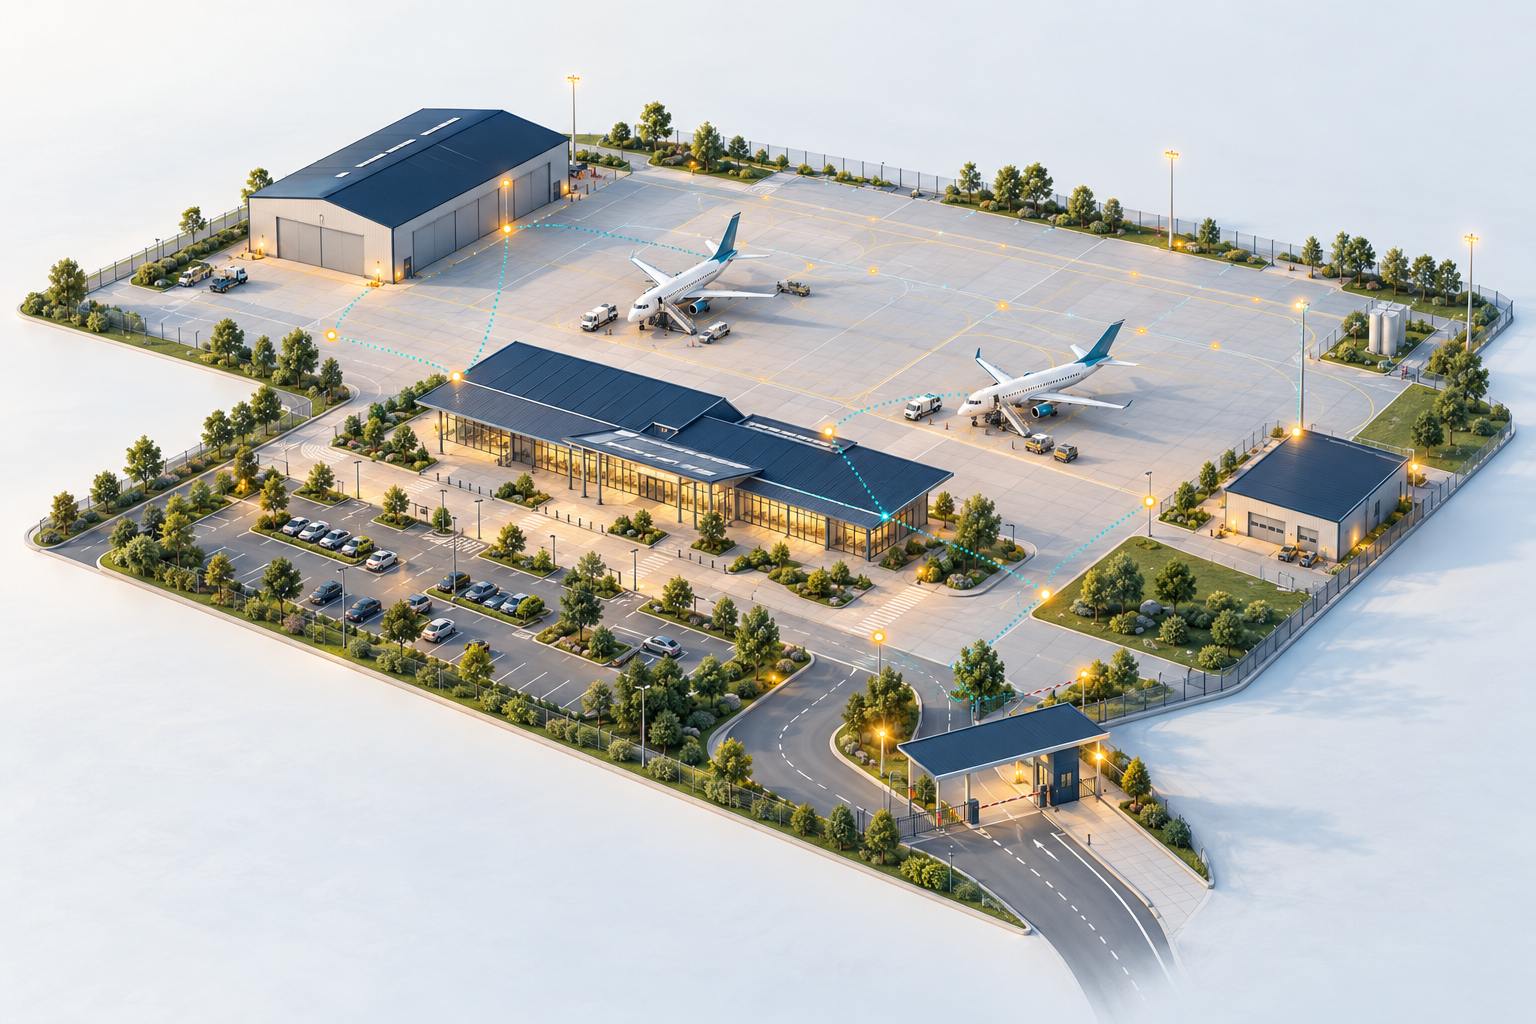
\includegraphics[width=\linewidth]{images/airport-cover.png}\par
{\scriptsize\color{muted}Wizualizacja koncepcyjna wygenerowana przez AI. Układ poglądowy; obowiązują rysunki techniczne w rozdziale 6.}\par
\vfill
\begin{tabularx}{\linewidth}{@{}Y r@{}}
\uczelnia & \dataprojektu\\
\autorzy & Wersja \wersja\\
\prowadzacy & Obiekt fikcyjny
\end{tabularx}\par
\vspace{3mm}
{\small\color{muted}Zakres: strefa terminalowo-techniczna. Koncepcja akademicka do konsultacji i dalszego projektowania.}\par
\end{titlepage}
\setcounter{page}{2}
